%%%%%%%%%%%%%%%%%%%%%%%%%%%%%%%%%%%%%%%%%%%%%%%%%%
%%%%%%%%%%%%%%%%%%%%%%%%%%%%%%%%%%%%%%%%%%%%%%%%%%
%%
%% Based one the "beamer-greek-two" template provided 
%% by the Laboratory of Computational Mathematics, 
%% Mathematical Software and Digital Typography, 
%% Department of Mathematics, University of the Aegean
%% (http://myria.math.aegean.gr/labs/dt/)
%%
%% Adapted by John Liaperdos, October-November 2014
%% (ioannis.liaperdos@gmail.com)
%%
%% Last update: 22/06/2017 (English Support)
%%
%%%%%%%%%%%%%%%%%%%%%%%%%%%%%%%%%%%%%%%%%%%%%%%%%%
%%%%%%%%%%%%%%%%%%%%%%%%%%%%%%%%%%%%%%%%%%%%%%%%%%
%%
\PassOptionsToPackage{unicode}{hyperref}
\PassOptionsToPackage{naturalnames}{hyperref}
\documentclass{beamer} 
%\usepackage{babel}
%\usepackage[utf8]{inputenc}


%%% FONT SELECTION %%%%%%%%%%%%%%%%%
%%% we choose a sans font %%%%%%%%%%
\usepackage{kmath,kerkis}
\usepackage[utf8]{inputenc} 
%\usepackage[default]{gfsneohellenic} 
%%%%%%%%%%%%%%%%%%%%%%%%%%%%%%%%%%%%

\usepackage{color}
\usepackage{amsmath}
\usepackage{amssymb}

\usepackage{epstopdf}
\usepackage{graphicx}
\graphicspath{{./images/}}

%%
% load TEI-Pel - specific layout
\usepackage{TeiPel_En_Beamer_Layout}
\setTeipelLayout{draft,newlogo}% options: "draft", "newlogo"

%%%%%%%%%%%%%%%%%%%%%%%%%%%%%%%%%%%%%%%%%%%%%%%%%%%%%%%%%%%%
% Thesis Info %%%%%%%%%%%%%%%%%%%%%%%%%%%%%%%%%%%%%%%%%%%%%%
%%%%%%%%%%%%%%%%%%%%%%%%%%%%%%%%%%%%%%%%%%%%%%%%%%%%%%%%%%%%
	% title
		\title[Modelo de sistema  de apoyo al diagnóstico de melanoma utilizando redes convolucionales]{Modelo de sistema  de apoyo al diagnóstico de melanoma utilizando redes convolucionales}	
	% author 
    % (In the mandatory argument "{}", separate multiple
    % authors with "\and" - use "\\" for better author name formatting
    % in the title page. In the optional argument "[]" include all
	% author names, with no "\and" or text formatting macros.)
	% Example: 
    %\author[A. Author Albert Einstein]{Anthony Author \and Albert Einstein}
		\author[A. Author]{Pablo Fernando Guzman Quispe}
	% supervisor	
	%	\supervisor{Supervisor}{Mister Supervisor}{Professor}
	% date
		\presentationDate{Octubre 23, 2017}
%%%%%%%%%%%%%%%%

\begin{document}

% typeset front slides
	\typesetFrontSlides

%%%%%%%%%%%%%%%%
% Your Slides Start here:

%%%%
\section{Descripción de la Realidad del Problema}
\tableofcontents[currentsection,currentsubsection] 
\begin{frame}{¿Que es el Melanoma?}

\begin{itemize}
	\item El melanoma es el tipo de cáncer de piel más mortífera. A pesar de esto sólo representa el 4\% de todos los cánceres de piel, que causa el 75\% de todos los casos de muerte.

	\item Es una de la más fáciles de curar, solo si es detectado en etapas muy tempranas
	
	\item Si es detectado muy tarde lo más probable es que haya penetrado a dentro de la piel con riesgo de metástasis.
	
\end{itemize}
\end{frame} 

\begin{frame}{¿Como se detecta?}
\begin{itemize}
	\item Clinico: Se basa en la experimencia del médico para la detección del melonoma.
	
	\item Biopsia: Extraccion de la lesion y analisis, puede provocar un deteriro mas rapido. Es costoso.
	
	\item Dermastoscopia: imagenes de una optima resolucion y enfocado a la lesion en la piel para el diagnostico segun el juicio del médico.
	
	\item AutoDeteccion: Se promueve la tecnica para toda la poblacion, pero solo un especialista da el diagnostico.

	
\end{itemize}
\end{frame} 

\begin{frame}{¿Cual es el problema?}

\begin{itemize}
	\item No todos las personas tiene los medios economicos para pagar unos de los metodos
	
	\item Solo un especialista puede dar el diagnostico de melanoma
	
	\item Melanoma es un tipo de cancer muy común.
	
\end{itemize}
\end{frame} 

%%%%
%
\section{Formulación del Problema}
\tableofcontents[currentsection,currentsubsection] 
\subsection{Problema}
\begin{frame}{Propuesta}
Conociendo los métodos de diagnosis de melanoma existentes. Es posible crear un método de diagnóstico con visión computacional utilizando los algoritmos de aprendizaje automático \textbf{\textit{Deep Learning}} para el clasificador.
\end{frame}

\subsection{Solución}
\begin{frame}{Esquema}
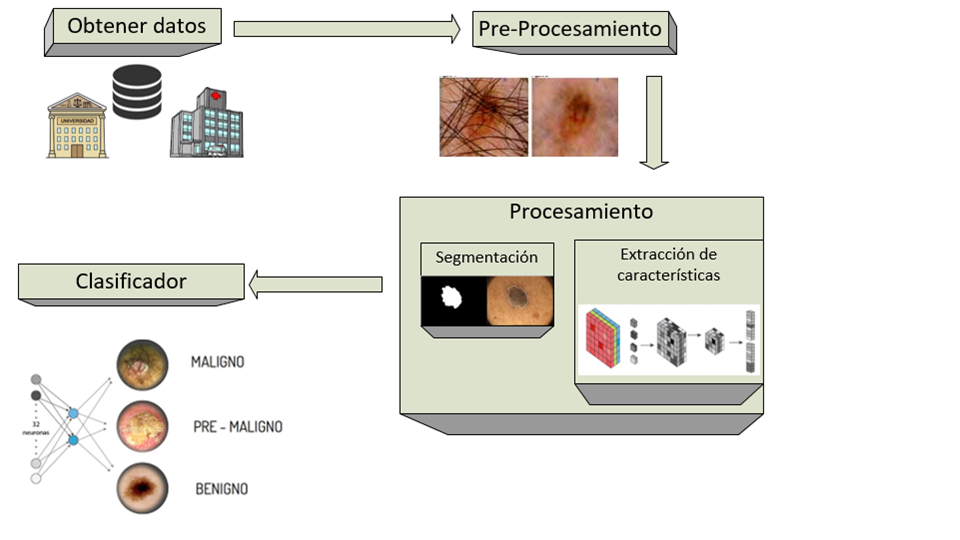
\includegraphics[width=1.1\textwidth]{images/esquema_v01.png}
\end{frame}

\section{Objetivos del Problema}
\tableofcontents[currentsection,currentsubsection] 

\subsection{Objetivo General}

\begin{frame}{Objetivo General}
Proponer un sistema de identificación de melanomas utilizando como clasificador los algoritmos de aprendizaje automático llamado \textbf{\textit{Deep Learning}}, puede tener resultados más precisos que los sistemas ya existentes.
\end{frame}

\subsection{Objetivos Específicos}

\begin{frame}{Objetivos Específicos}
Los objetivos son los siguientes:
\begin{itemize}
	\item Investigar estado del arte del tema.
	\item Investigar melanoma y sus diagnósticos
	\item Investigar sobre deeplearning y el diagnóstico
	\item Proponer los elementos constitutivos del modelo
	\item Evaluar y validar el modelo
	
\end{itemize}
\end{frame}

\section{Resultados}
\tableofcontents[currentsection,currentsubsection] 
\subsection{Resultados de análisis}

\begin{frame}{Primeros resultados}

\begin{itemize}
	\item En construcción
\end{itemize}
\end{frame}



\section{Cronograma}
\tableofcontents[currentsection,currentsubsection] 

\subsection{cronograma}

\begin{frame}{cronograma}
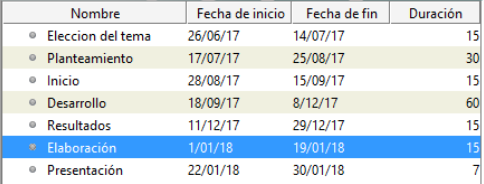
\includegraphics[width=1.1\textwidth]{images/cronograma.png}
\end{frame}

\section{Código}
\tableofcontents[currentsection,currentsubsection] 

\subsection{código}

\begin{frame}{Carga}
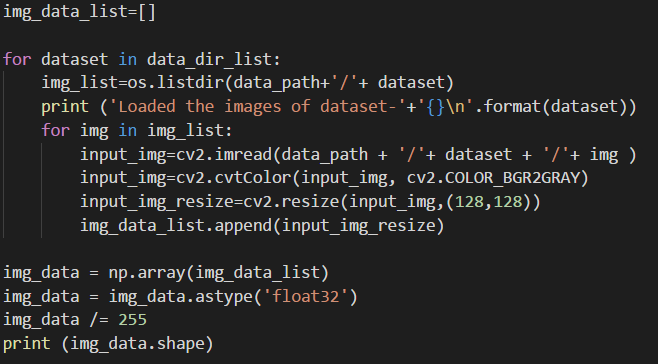
\includegraphics[width=1.1\textwidth]{images/carga.png}
\end{frame}

\begin{frame}{división de data}
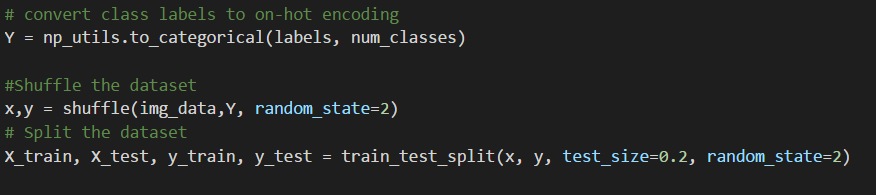
\includegraphics[width=1.1\textwidth]{images/division.png}
\end{frame}

\begin{frame}{Modelo Definición}
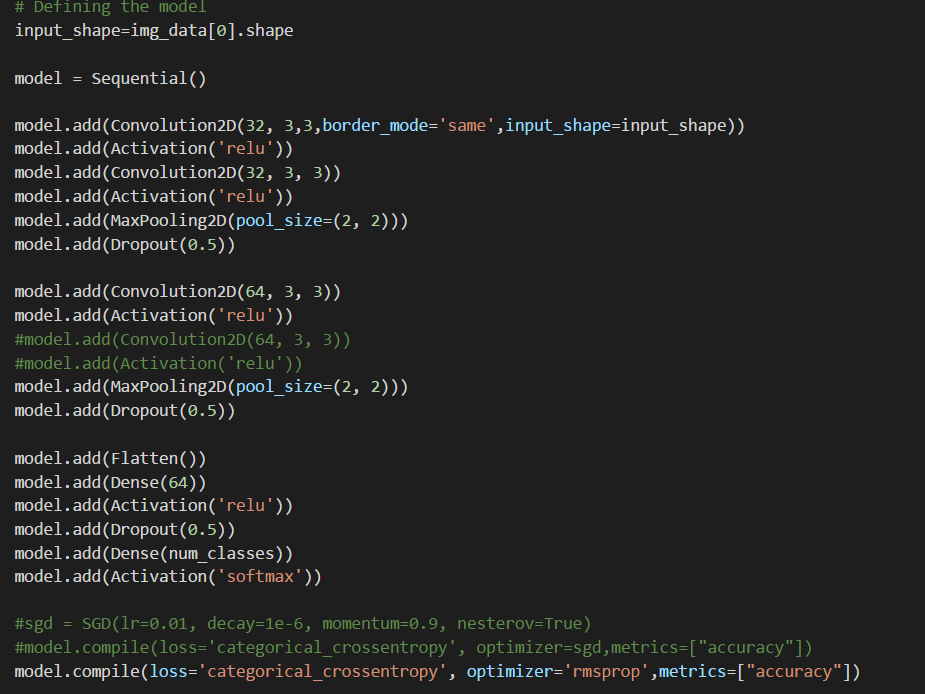
\includegraphics[width=1.1\textwidth]{images/definicion_modelo.png}
\end{frame}

\section{Repositorio}
\tableofcontents[currentsection,currentsubsection] 

\subsection{Git}

\begin{frame}{GitHub}
https://github.com/guzman890/tesis-melanoma-dl.git
\end{frame}

%\begin{frame}{References}
%	\begin{thebibliography}{2}
%	\beamertemplatebookbibitems
%	\bibitem{Author1990}A.\ Author. \newblock\emph{Handbook of Everything}.\newblock
%	\textlatin{Some Press, \oldstylenums{1990}}.
%
%	\beamertemplatearticlebibitems
%	\bibitem{Someone2002}B.\ Author.\newblock On this and that\emph{.}
%	\newblock\emph{Journal on This and That}. 
%	\oldstylenums{2}(\oldstylenums{1}):\oldstylenums{50}--\oldstylenums{100}, 
%	\oldstylenums{2000}.
%	\end{thebibliography}
%\end{frame}

%%
\end{document}